\section{Sizing}\label{sizing}

A fundamental question is how large the LSST Data Management System must be. To
this end, a complex analytical model has been developed driven by input from
the requirements specifications. Specifications from the science requirements
and other subsystem designs, and the observing strategy, translate directly
into numbers of detected sources and astronomical objects, and ultimately into
required network bandwidths and the size of storage systems. Specific science
requirements of the survey determine the data quality that must be maintained
in the DMS products, which in turn determine the algorithmic requirements and
the computer power necessary to execute them. The relationship of the elements
of this model and their flow-down from systems and DMS requirements is shown in
Figure \ref{fig:sizing-model}. Detailed sizing computations and associated
explanations appear in LSST Documents listed on the Figure.

\begin{figure}
\centering
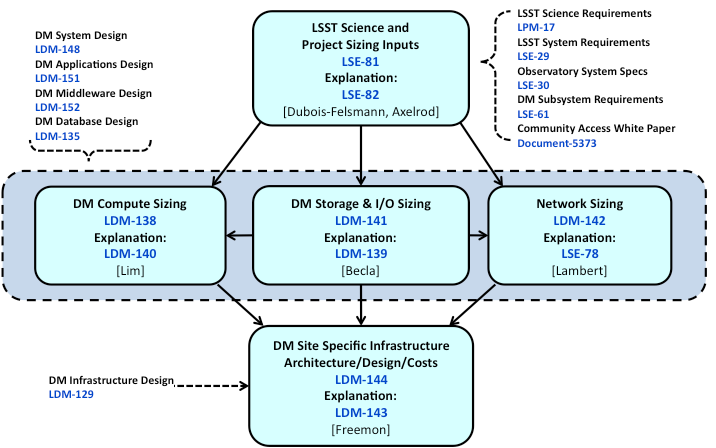
\includegraphics[width=\textwidth]{SizingModel.png}
\caption{DMS Infrastructure Sizing and Estimation}
\label{fig:sizing-model}
\end{figure}

Key input parameters include camera characteristics, the expected cadence of
observations, the number of observed stars and galaxies expected per band, the
processing operations per data element, the data transfer rates between and
within processing locations, the ingest and query rates of input and output
data, the alert generation rates, and latency and throughput requirements for
all data products.

Processing requirements were extrapolated from the functional model of
operations, prototype pipelines and algorithms, and existing precursor
pipelines adjusted to LSST scale.  As a part of every Data Release, all data
previously processed are reprocessed with the latest algorithms, calibration
products, and parameters. This causes the processing requirements to increase
with time.  Advances in hardware performance, however, are expected to reduce
the number of nodes needed and the power and cooling devoted to them. This causes some of the performance figures in Table \ref{table:compute-sizing} to reach
a high-water mark during the survey.

\begin{center}
\begin{longtable}{|c|c|c|c|}
\caption{DMS Compute Infrastructure Sizing; growth from Survey Year 1 to Year 10; hwm = high-water mark \label{table:compute-sizing}}\\   %%%% need this line break for caption
 \hline
	& & \textit{Archive Site} & \textit{Base Site} \\ \hline
\multirow{4}{*}{Compute} & TeraFLOPS (sustained) & 197 $\rightarrow$ 970 & 30 $\rightarrow$ 62 \\ \cline{2-4}
  & Nodes & 436 $\rightarrow$ 305 (455 hwm) & 56 $\rightarrow$ 17 (59 hwm) \\ \cline{2-4}
  & Cores & 18K $\rightarrow$ 62K & 3K $\rightarrow$ 4K \\ \hline
\multirow{2}{*}{Database} & TeraFLOPS (sustained) & 40 $\rightarrow$ 310 & 55 $\rightarrow$ 306 \\ \cline{2-4}
  & Nodes & 94 $\rightarrow$ 113 (148 hwm) & 108 $\rightarrow$ 98 (133 hwm) \\ \cline{2-4}
\multirow{3}{*}{Facilities} & Floor Space & 826 $\rightarrow$ 744 ft$^2$ (834 hwm) & 278 $\rightarrow$ 195 ft$^2$ (435 hwm) \\ \cline{2-4}
  & Power & 274 $\rightarrow$ 273 kW (309 hwm) & 158 $\rightarrow$ 248 kW (248 hwm) \\ \cline{2-4}
  & Cooling & 0.9 $\rightarrow$ 0.9 mmbtu (1.1 hwm) & 0.5 $\rightarrow$ 0.8 mmbtu (0.8 hwm) \\ \hline
\end{longtable}
\end{center}

Storage and input/output requirements were extrapolated from the data model of
LSST data products, the DMS and precursor database schemas, and
existing database management system overhead factors in precursor
surveys and experiments adjusted to LSST scale. A summary of key numbers is
in Table \ref{table:storage-sizing}.

\begin{longtable}{|c|c|c|c|}
\caption{DMS Storage Infrastructure Sizing; growth from Survey Year 1 to Year 10 \label{table:storage-sizing}}\\
\hline
	& & \textit{Archive Site} & \textit{Base Site} \\ \hline
\multirow{3}{*}{File Storage} & Capacity & 24 $\rightarrow$ 81 PB & \\ \cline{2-4}
  & Drives & 1602 $\rightarrow$ 862 & 597 $\rightarrow$ 249 \\ \cline{2-4}
  & Bandwidth & 493 $\rightarrow$ 714 GB/s (752 hwm) & 223 $\rightarrow$ 231 GB/s (236 hwm) \\ \hline
\multirow{3}{*}{Database} & Capacity & 29 $\rightarrow$ 99 PB & 16 $\rightarrow$ 72 PB \\ \cline{2-4}
  & Drives & 3921 $\rightarrow$ 2288 & 2190 $\rightarrow$ 1642 \\ \cline{2-4}
  & Bandwidth & 1484 $\rightarrow$ 2040 GB/s (2163 hwm) & 829 $\rightarrow$ 1169 GB/s (1615 hwm) \\ \hline
\multirow{3}{*}{Tape Storage} & Capacity & 31 $\rightarrow$ 242 PB & \\ \cline{2-4}
  & Tapes & 2413 $\rightarrow$ 3691 (4117 hwm) & \\ \cline{2-4}
  & Tape Bandwidth & 36 $\rightarrow$ 65 GB/s & \\ \hline
\end{longtable}


Communications requirements were developed and modeled for the data transfers
and user query/response load, extrapolated from existing surveys and adjusted
to LSST scale.  These requirements are illustrated in Figures \ref{fig:near-real-time-flows} for per-visit transfers and Figure \ref{fig:annual-reprocessing-flows} for annual transfers.  Peak bandwidths assume 5 seconds for international
image transfer and 30 days to transfer Data Release catalogs from NCSA to the
Chilean DAC.

\begin{figure}
\centering
\includegraphics[width=\textwidth]{images/NearRealTimeDataFlow.pdf}
\caption{Near Real-Time Data Flows}
\label{fig:near-real-time-flows}
\end{figure}

\begin{figure}
\centering
\includegraphics[width=0.5\textwidth]{images/AnnualReprocessingDataFlow.pdf}
\caption{Annual Reprocessing Data Flows}
\label{fig:annual-reprocessing-flows}
\end{figure}

In all of the above, industry-provided technology trends (\citeds{LDM-143})
were used to extrapolate to the LSST construction and operations phases in
which the technology will be acquired, configured, deployed, operated, and
maintained. A just-in-time acquisition strategy is employed to leverage
favorable cost/performance trends.

The resulting performance and sizing requirements show the DMS to be a
supercomputing­-class system with correspondingly large data input/output and
network bandwidth rates.  Despite this size, technology trends show this to be
well within the anticipated performance of commodity-based systems during the
construction and operations time frame.

